\section{Méthodologie}
\begin{frame}{Mise en main}
\centering
	\only<1,2,4,5>{
		\begin{itemize}
	\item<1,2,4,5> Software \powerfactory
	\begin{itemize}
		\item<2,4,5> Interface
		\item<4,5> Exemples pour apprendre\note<4>{Lembrar de falar dos scripts e linguagens\\Também dos tipos de Simulação}
		\item<5> Montage modèle du réseau
	\end{itemize}
	\end{itemize}
}
	\only<3>{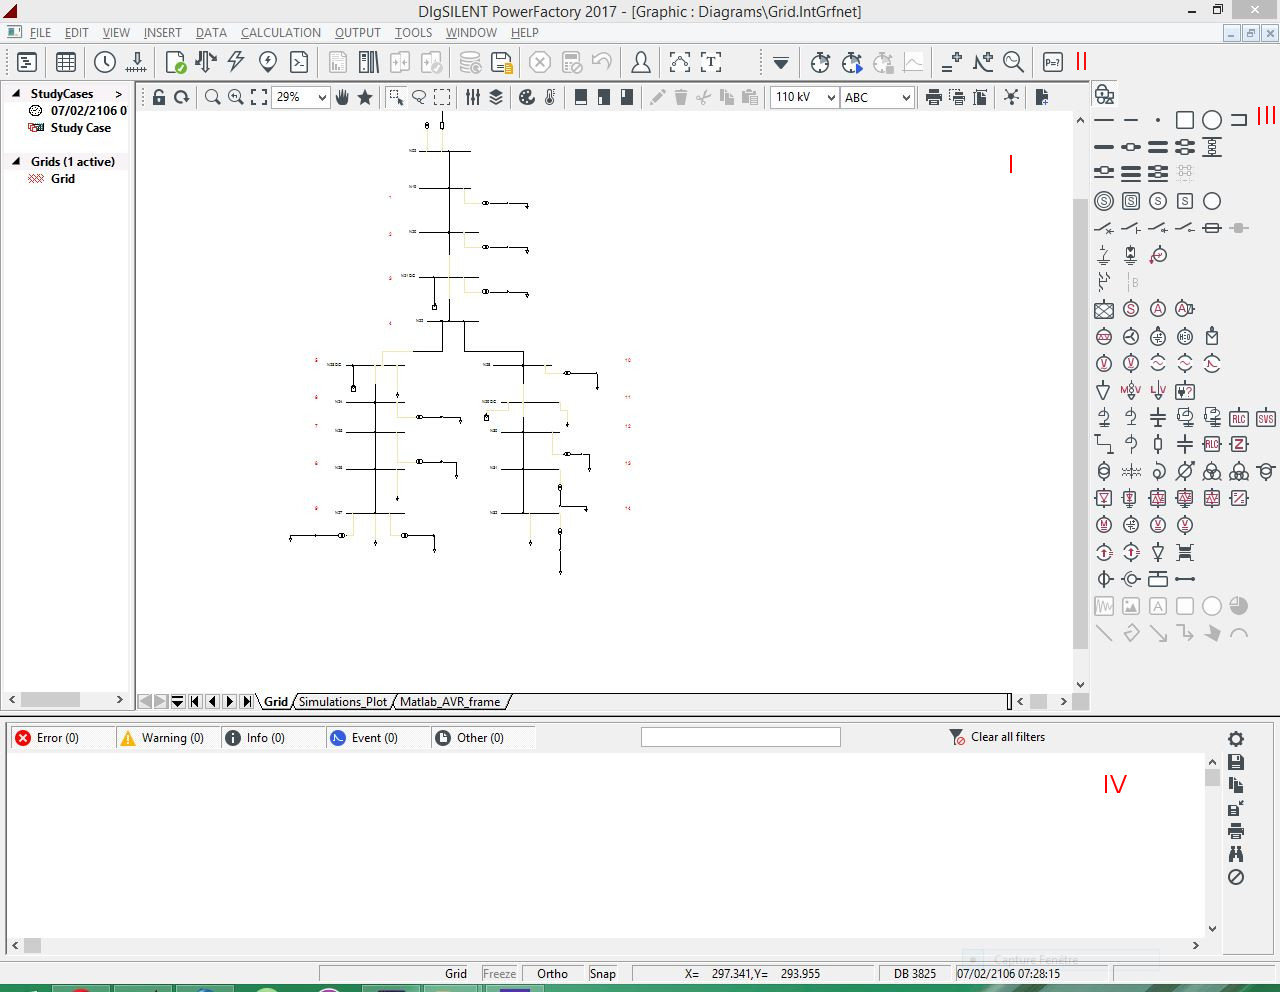
\includegraphics[width=0.7\textwidth]{Methodologie/partie_2/gui_powerfactory_num.JPG}}
\only<6>{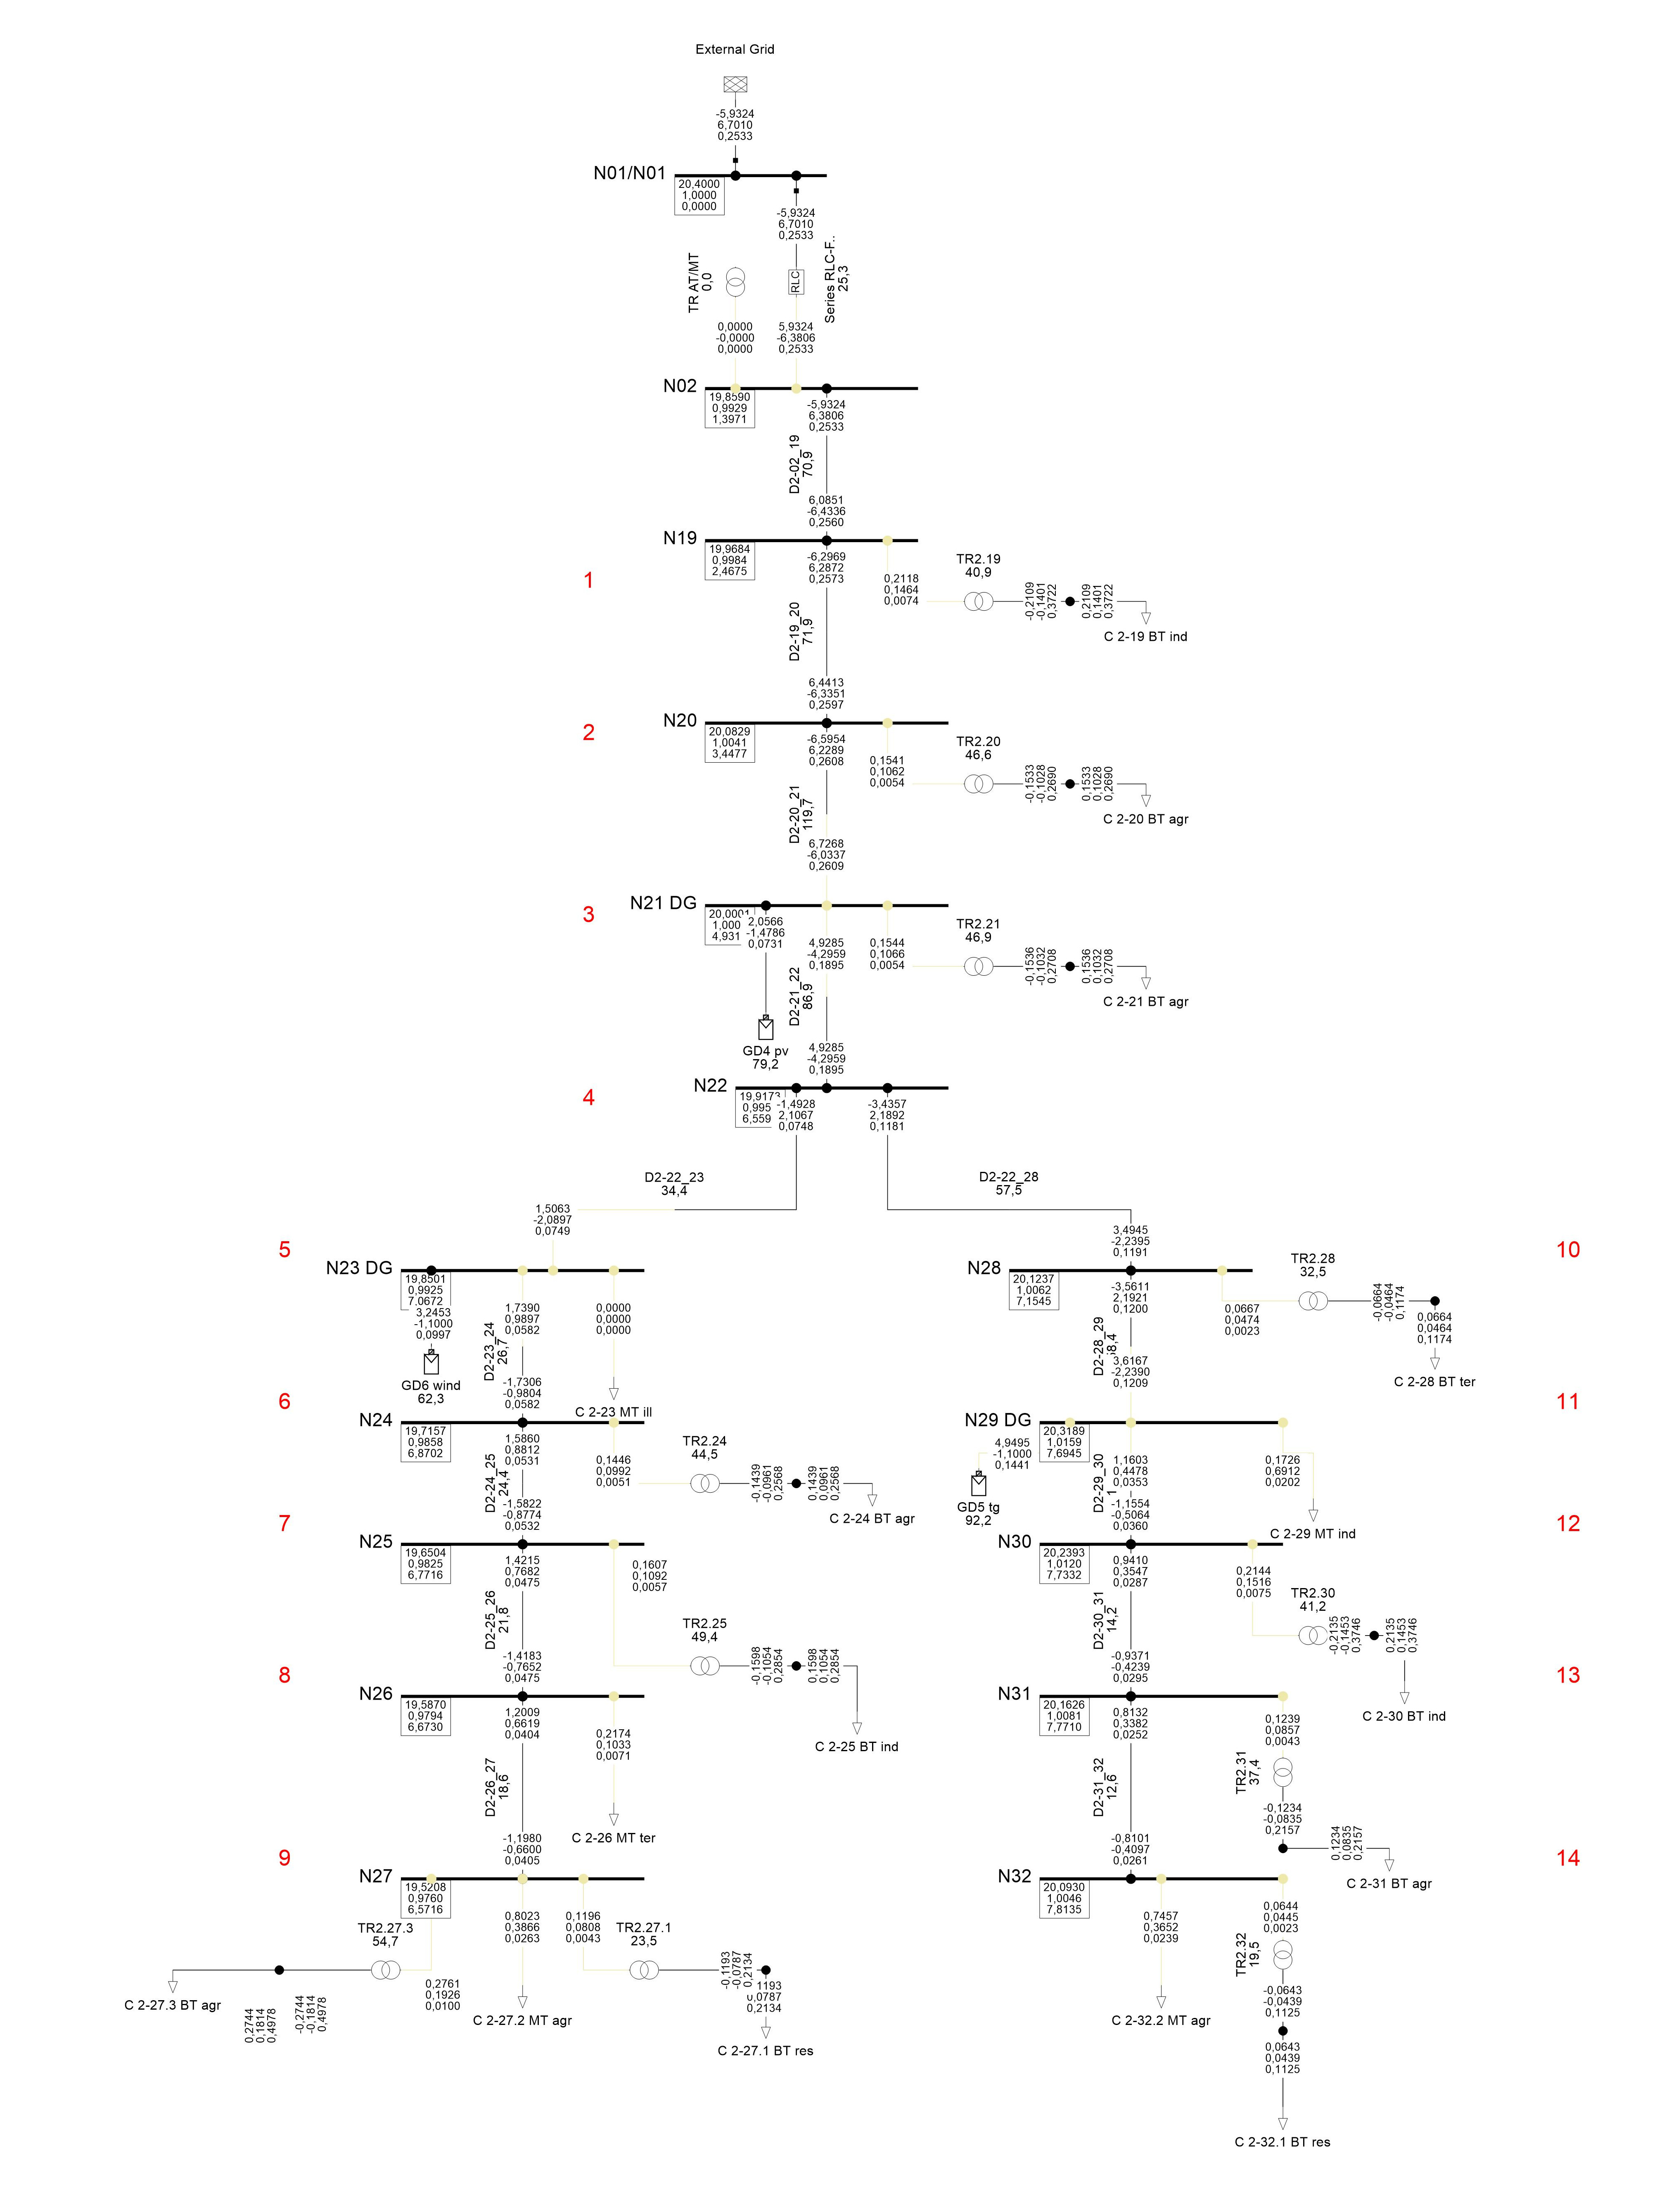
\includegraphics[height=0.8\textheight]{Methodologie/Diagramme_du_reseaux}}
	
\end{frame}

\begin{frame}{Programmation}
Scripts en MATLAB et Python:\pause
	\begin{itemize}
		\item Charger valeurs dans le modèle\pause
		\item Calculer gains\pause
		\item Créer événements qui se passent pendant les simulations\pause
		\item Faire des simulations RMS et EMT\pause
		\item Prendre les données \texttt{.csv} en \texttt{.mat}\pause
	\end{itemize}
\end{frame}

\begin{frame}{Intégration}
	Matlab/Simulink $ \leftrightarrow $ \powerfactory\pause
	\begin{itemize}
		\item Modèle Simulink \texttt{.mdl}\pause
		\item Fichier MATLAB \texttt{.m}\pause
		\item Bloc générique dans \powerfactory\  
	\end{itemize}
	\note<1>{Intégration pour faciliter modifier type de régulateur}
	\note<2>{Simulink onde fica o controlador}
	\note<3>{Matlab faz appel para courir simulação}
	\note<4>{Bloc crée dans \powerfactory qui appelle fichier .m\\Falar do problema de échantillonnage}
\end{frame}
\begin{frame}{Intégration}
\centering
\begin{tabular}{ccc}
	&$ \downarrow $&\\
	\rotatebox[origin=c]{90}{ $ \Lsh $} & PowerFactory &$ \Lsh $ \\ 
	MATLAB&  &MATLAB  \\ 
	 \rotatebox[origin=c]{180}{ $ \Lsh $}  &Simulink&\rotatebox[origin=c]{270}{ $ \Lsh $} 
\end{tabular} 
\end{frame}
